\documentclass[10pt,aspectratio=169]{beamer}
\usepackage[utf8]{vietnam}
\usepackage{fil}

\title{Tìm hiểu cơ bản về Reinforcement Learning và Gymnasium}
\subtitle{Future Internet Laboratory}
\author{Nguyễn Phạm Trung Hiếu}

\begin{document}

\maketitle

\begingroup
    \begin{frame}{Nội dung chính}{}
        \tableofcontents
    \end{frame}
\endgroup

\section{Tìm hiểu về Reinforcement Learning}

\subsection{Reinforcement Learning là gì?}

\begin{frame}{Reinforcement Learning là gì?}
\textbf{Ví dụ 1:} Việc huấn luyện một con chó bằng phần thưởng:
\begin{itemize}
\setlength\itemsep{8pt}
\item Nhiệm vụ được đưa ra là huấn luyện một con chó cư xử đúng mực, điều này không thể chứng minh được bằng việc huấn luyện nhiều con chó (tương đương với một tập hợp các mẫu).
\item Phương pháp là để con chó tự do hành động, mỗi khi nó làm điều gì tốt thì khen và cho nó một phần thưởng, ngược lại, phạt nó mỗi khi nó làm điều gì xấu.
\item[] $ \longrightarrow $ Con chó sau đó sẽ tự nhận biết được điều tốt và điều xấu
\item[] $ \longrightarrow $ Cơ sở đào tạo của thuật toán \textcolor{mainblue}{\textit{reinforcement learning}}
\end{itemize}
\end{frame}

\begin{frame}{Reinforcement Learning là gì?}
\textbf{Ví dụ 2:} Một chiếc máy bay tự động có thể tự bay bằng cách sử dụng RL:
\begin{itemize}
\setlength\itemsep{8pt}
\item Nhiệm vụ được đưa ra là xác định vị trí của chiếc máy bay, từ đó quyết định cách di chuyển cần của của bộ điều khiển.
\begin{itemize}
\setlength\itemsep{4pt}
\item[-] Vị trí, hướng, tốc độ... của máy bay được gọi là \textbf{state $ \boldsymbol{s} $} (trạng thái)
\item[-] Việc quyết định cách di chuyển của bộ điều khiển được gọi là \textbf{action $ \boldsymbol{a} $} (hành động) 
\end{itemize}
\item[] $ \longrightarrow $ Nhiệm vụ lúc này là tìm một hàm ánh xạ từ state $ s $ sang action $ a $, tương ứng với việc di chuyển hai cần điều khiển như thế nào để giữ cho máy bay thăng bằng trên không mà không rơi.
\item Thay vì là một tập hợp các mẫu, đầu vào chính trong \textcolor{mainblue}{\textit{reinforcement learning}} được gọi là \textbf{reward} (phần thưởng) hay \textbf{hàm reward}, định nghĩa cho máy bay biết khi nào nó đang hoạt động tốt và khi nào hoạt động kém.
\end{itemize}
\end{frame}

\begin{frame}{Reinforcement Learning là gì?}
\textbf{Định nghĩa:} \textcolor{mainblue}{\textit{Reinforcement learning}} là phương pháp đào tạo các mô hình học máy để đưa ra một chuỗi các quyết định hay hành động phù hợp để đạt được kết quả tốt nhất trong một tình huống cụ thể. Trong RL, dữ liệu được tích lũy từ chính các hệ thống học máy sử dụng phương pháp thử và sai (trial-and-error), nghĩa là ta định nghĩa được cho thuật toán biết phải làm gì hơn là làm như thế nào.\\
\vspace{12pt}
\textbf{Kết luận:}
\begin{itemize}
\setlength\itemsep{8pt}
\item Nhiệm vụ của thuật toán \textcolor{mainblue}{\textit{reinforcement learning}} là tìm ra cách thu được nhiều kết quả tốt hơn và ít kết quả xấu.
\item Trọng tâm của \textcolor{mainblue}{\textit{reinforcement learning}} là tìm kiếm sự cân bằng giữa khám phá (kiến thức chưa biết) và khai thác (kiến thức hiện tại)\footnotemark.
\end{itemize}
\footnotetext[1]{L. P. Kaelbling, M. L. Littman, and A. W. Moore, “Reinforcement Learning: A Survey,” \textit{Journal of Artificial Intelligence Research}, vol. 4, pp. 237–285, May 1996, doi: 10.1613/jair.301.}
\end{frame}

\subsection{Các thuật ngữ trong Reinforcement Learning}

\begin{frame}{Agent và environment}{\subsecname}
\begin{columns}
\begin{column}{0.4\textwidth}
\textbf{Agent} là thực thể quan sát môi trường và sinh ra hành động tương ứng.\\
\vspace{48pt}
\textbf{Environment} là không gian xung quanh của agent, nơi mà agent tồn tại và tương tác.\\
\end{column}
\begin{column}{0.5\textwidth}
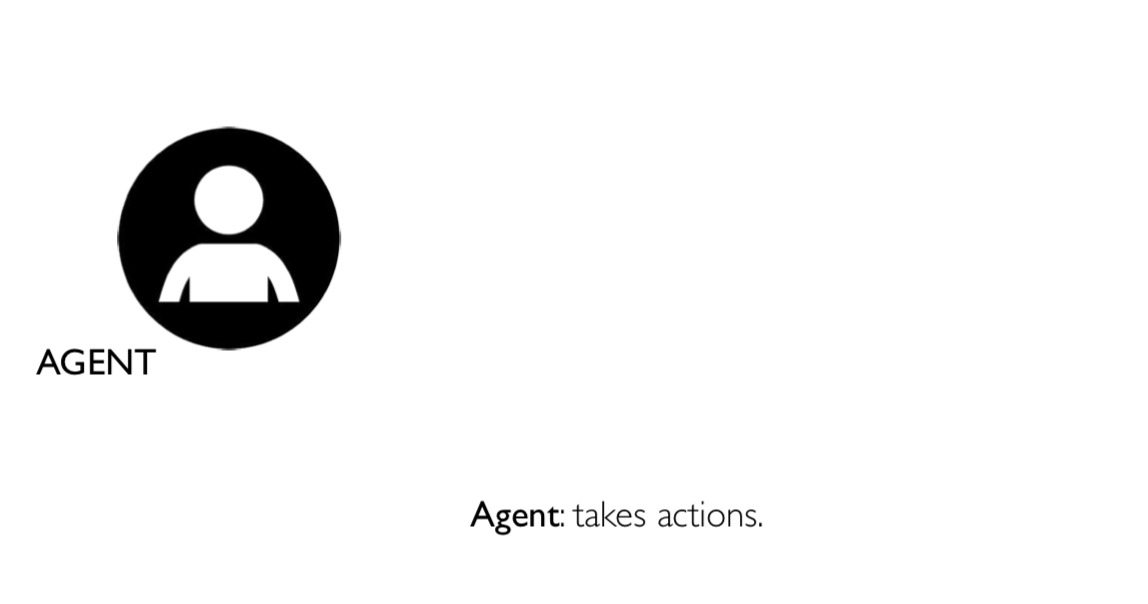
\includegraphics[width=\textwidth]{source/1.png}\\

\includegraphics[width=\textwidth]{source/2.png}\\
\end{column}
\end{columns}
\end{frame}

\begin{frame}{State, action và observation}{\subsecname}
\begin{columns}
\begin{column}{0.4\textwidth}
\textbf{Action $ \boldsymbol{a} $} là phương thức của agent cho phép nó tương tác với environment và thay đổi environment.\\
\vspace{8pt}
\textbf{State $ \boldsymbol{s} $} là trạng thái của environment mà agent nhận được.\\
\vspace{8pt}
$ \longrightarrow $ Dựa trên state $ s $ của environment hiện tại mà agent sẽ đưa ra action $ a $\\
\vspace{20pt}
\textbf{Observation} là hành động của environment sau khi nhận được sự tương tác từ agent, environment có sự chuyển đổi trạng thái đối với agent.\\
\end{column}
\begin{column}{0.5\textwidth}
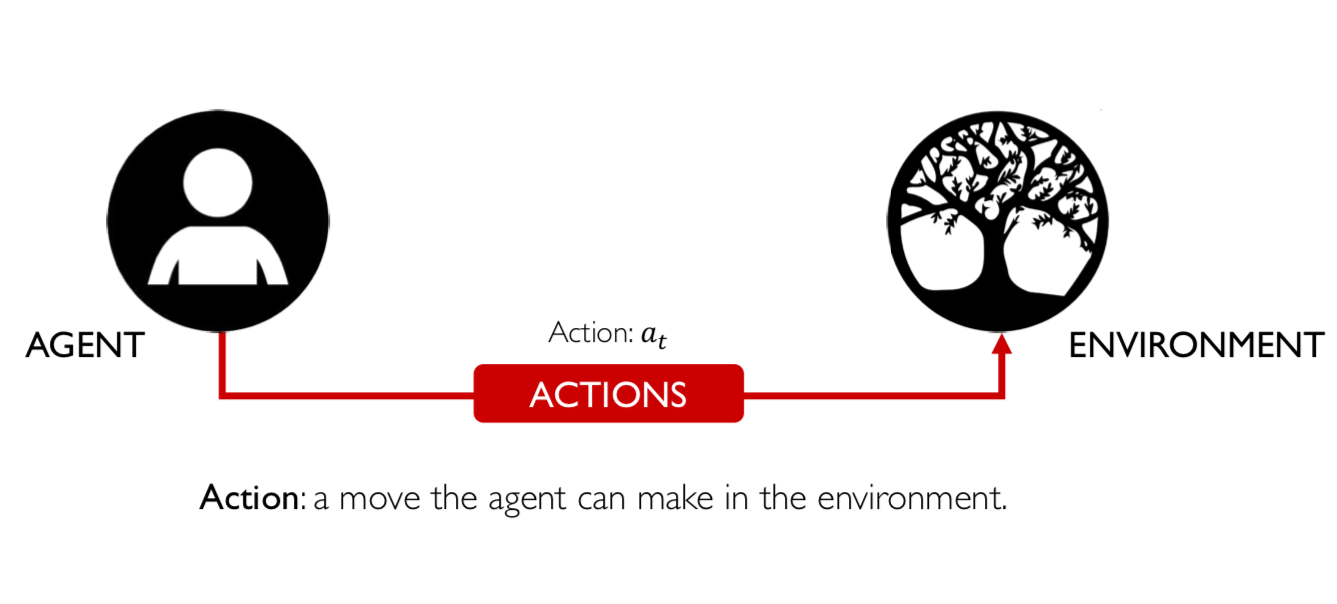
\includegraphics[width=\textwidth]{source/3.png}\\
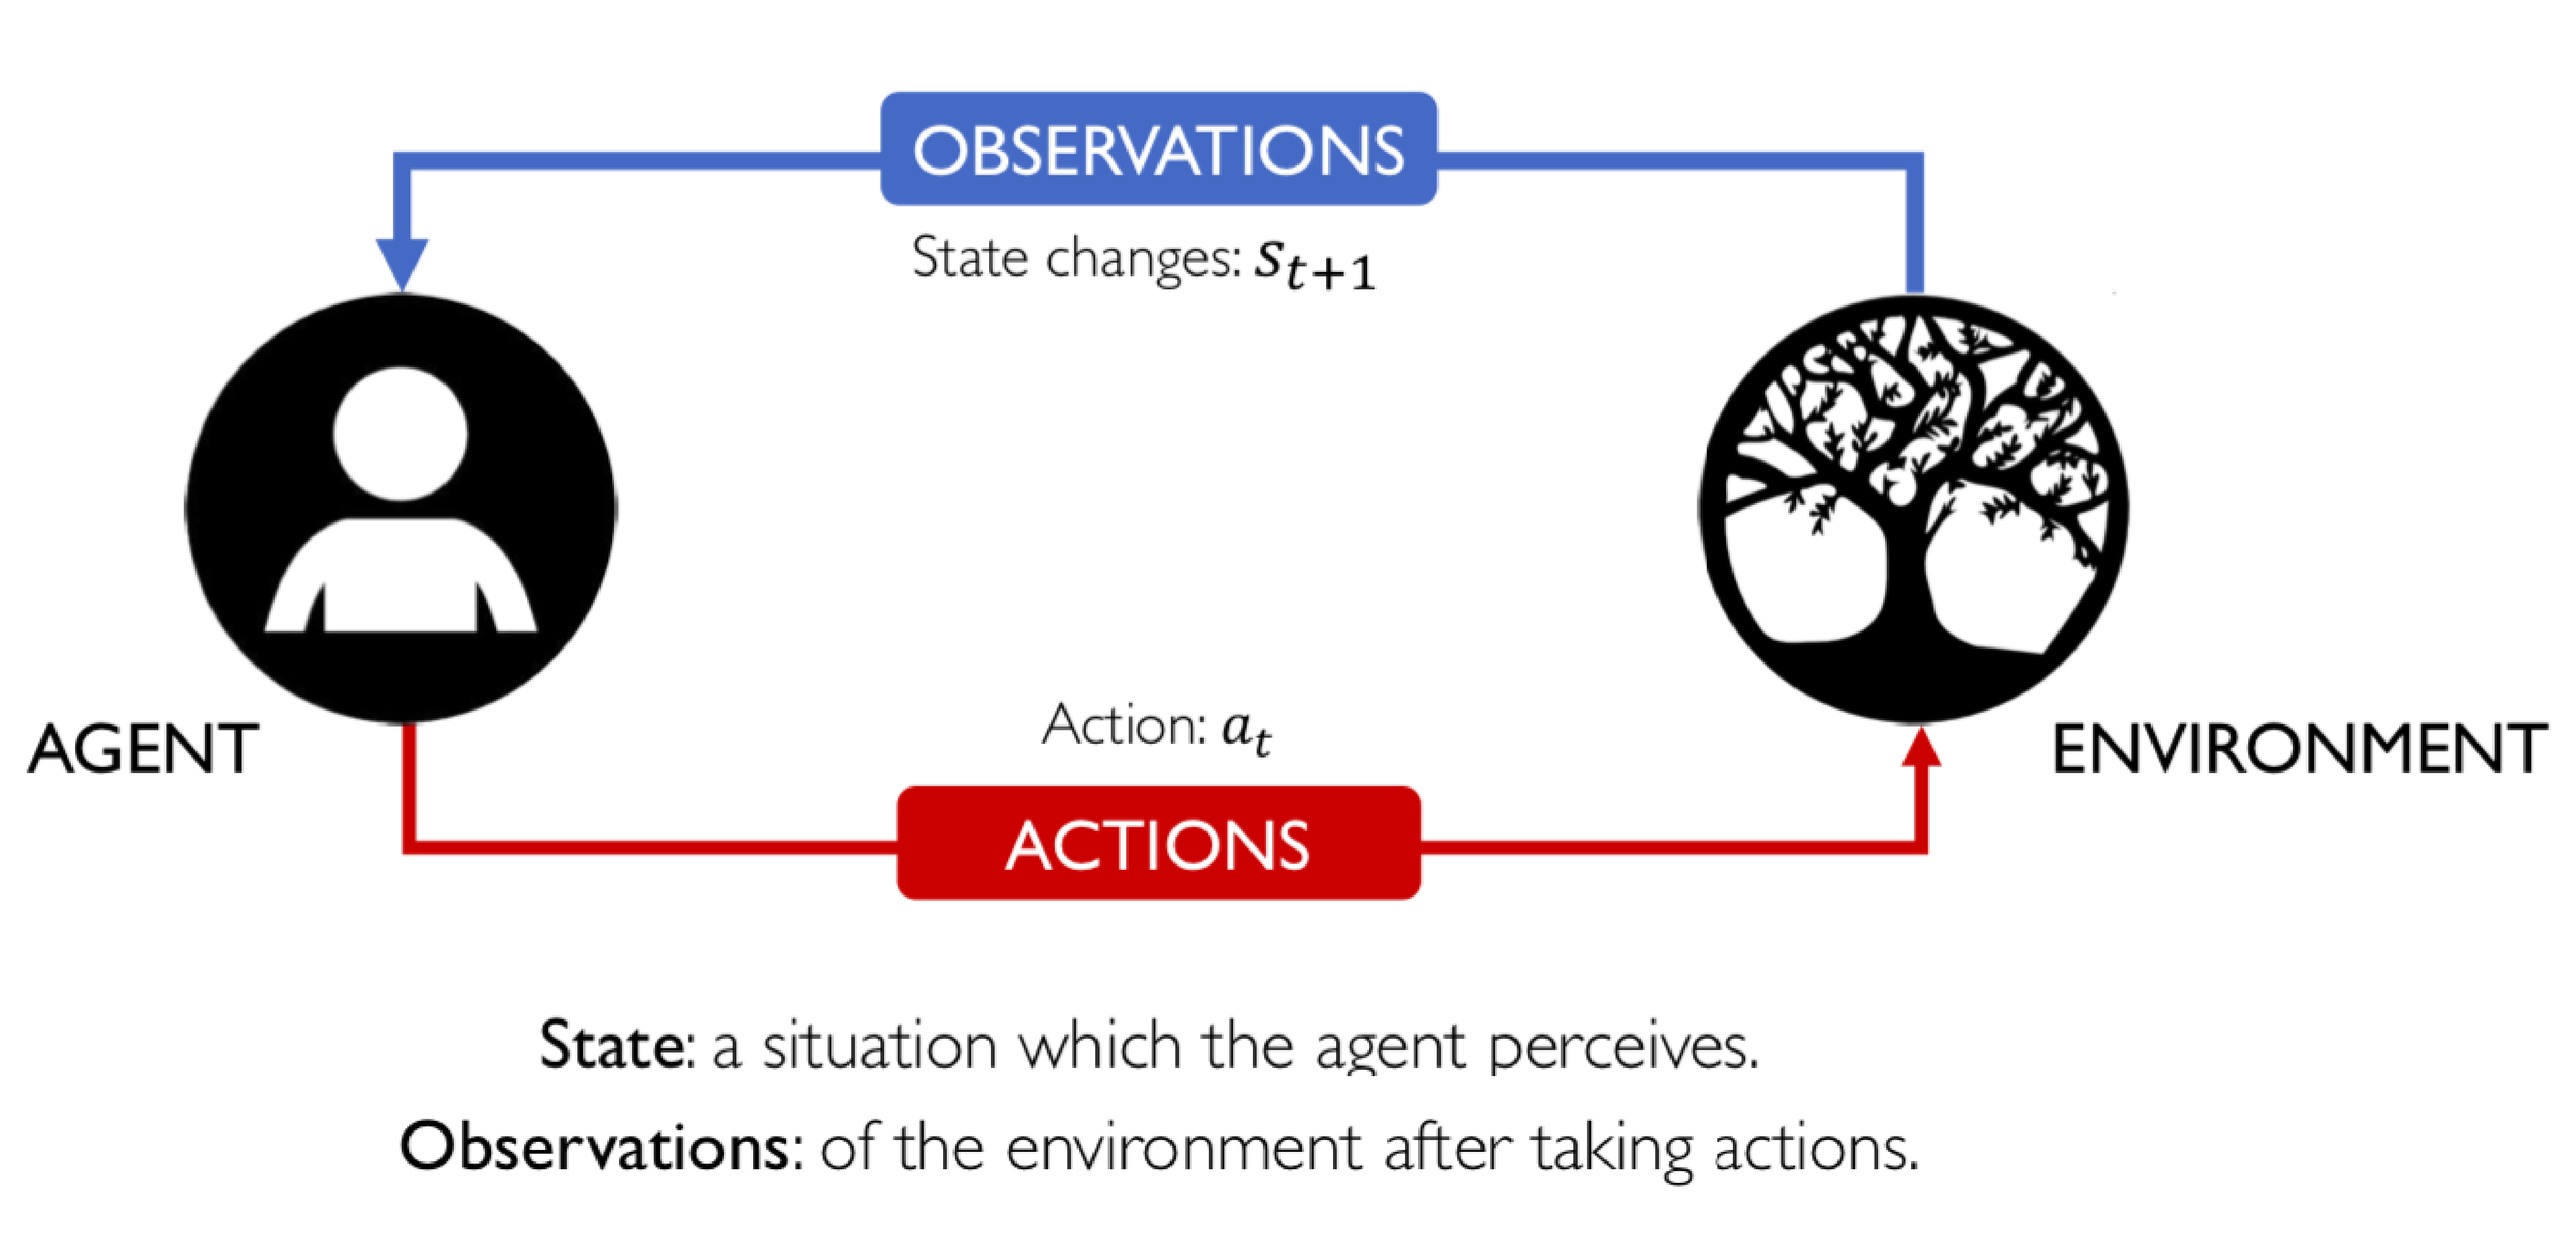
\includegraphics[width=\textwidth]{source/4.png}\\
\end{column}
\end{columns}
\end{frame}

\begin{frame}{Khái niệm reward}{\subsecname}
\begin{columns}
\begin{column}{0.4\textwidth}
Ở mỗi action, environment sẽ gửi đến cho agent một "phần thưởng" xác định. Mục tiêu của agent là tối đa hóa tổng "phần thưởng" mà nó nhận được trong một thời gian cụ thể. Tín hiệu "phần thưởng" (reward signal) giúp xác định đâu là action tốt và xấu đối với agent, đồng thời nó cũng là cơ sở chính để thay đổi policy. Nếu một action được lựa chọn bởi policy mang đến "phần thưởng" thấp, thì policy đó có thể bị thay đổi. Agent sẽ lựa chọn các action khác trong các tình huống tương tự ở tương lai.\\
\end{column}
\begin{column}{0.5\textwidth}
\hypertarget{loop}{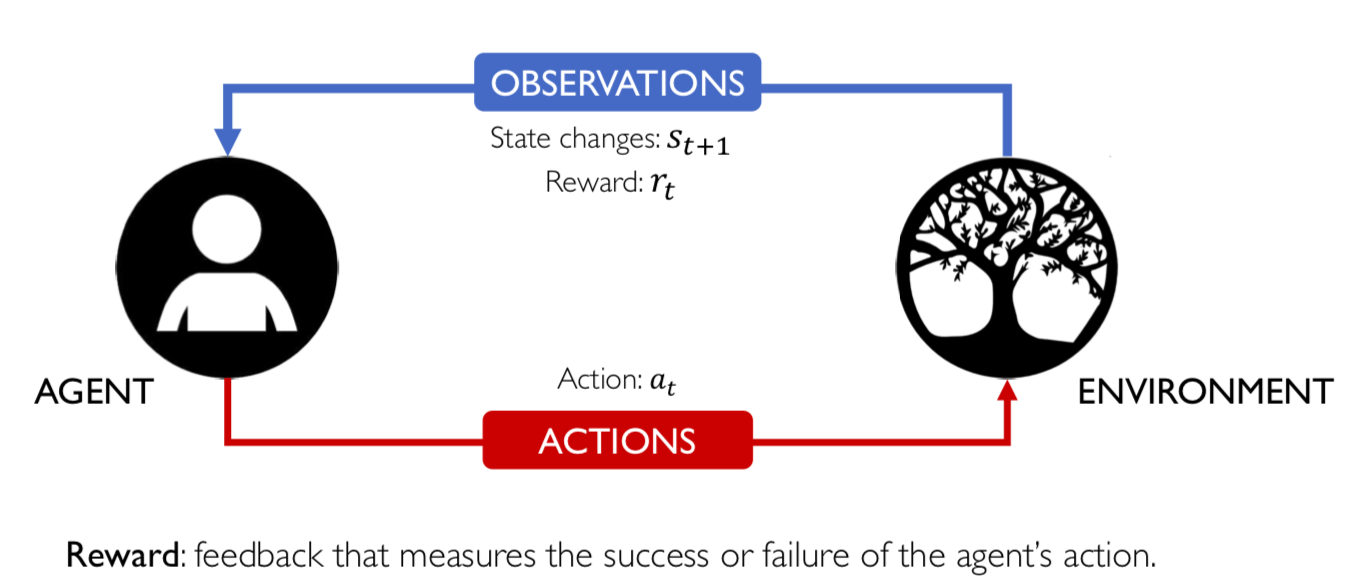
\includegraphics[width=\textwidth]{source/5.png}\\}
\vspace{20pt}
$ \longrightarrow $ \textbf{Reward $ \boldsymbol{R(s)} $} của state $ s $ là khái niệm định nghĩa cho agent biết khi nào nó đang hoạt động tốt và khi nào hoạt động kém\\
\end{column}
\end{columns}
\end{frame}

\begin{frame}{Khái niệm return}{\subsecname}
\begin{itemize}
\setlength\itemsep{8pt}
\item Với mỗi action được thực hiện, agent sẽ có các state khác nhau và nhận được các reward khác nhau $ \rightarrow $ \textbf{return} giúp xác định một nhóm reward cụ thể tốt hơn kém hơn một nhóm reward khác.
\item Khái niệm \textbf{return} cho thấy reward mà một agent nhận được sớm hơn có thể "hấp dẫn" hơn những reward mà agent mất nhiều thời gian để có được, hoặc ngược lại.
\item Giá trị của \textbf{return} được định nghĩa bằng tổng của các reward tại các state cho đến state kết thúc (terminal state) sau khi nhân với một trọng số $ \gamma $, được gọi là yếu tố suy giảm (discount factor) có giá trị gần bằng 1 (thường là 0.9, 0.99...)
\begin{equation*}
Return = \sum_{i=0}^{s_{terminal}} \gamma^i R(s_i) = R(s_0) + \gamma R(s_1) + \gamma^2 R(s_2) + ...
\end{equation*}
trong đó, $ R(s_i) $ là reward tại state $ s_i $ và $ s_{i+1} $ là state sau đó.
\end{itemize}
\end{frame}

\begin{frame}{Khái niệm return}{\subsecname}
\begin{itemize}
\setlength\itemsep{8pt}
\item Yếu tố suy giảm $ \gamma $ làm cho thuật toán RL trở nên "thiếu kiên nhẫn" (impatient), nghĩa là giá trị của các reward sẽ càng ít khi qua càng nhiều state, do đó, nhận được reward mong muốn càng sớm thì giá trị tổng "phần thưởng" hay return sẽ càng cao.
\item Giá trị \textbf{return} phụ thuộc vào reward, reward lại phụ thuộc vào action mà agent thực hiện
$ \rightarrow $ Giá trị \textbf{return} phụ thuộc vào action của agent
\item Đối với các hệ thống có reward nhỏ hơn 0, yếu tố suy giảm $ \gamma $ sẽ khiến thuật toán cố gắng đẩy reward này ra xa nhất có thể trong tương lai.
\end{itemize}
\end{frame}

\begin{frame}{Khái niệm policy}{\subsecname}
\begin{itemize}
\setlength\itemsep{8pt}
\item Trong RL, mục tiêu của ta là đưa ra một hàm được gọi là \textbf{policy $ \boldsymbol{\pi} $} giúp xác định cách thức hoạt động của agent tại một thời điểm nhất định, nói cách khác, nó là một ánh xạ từ các state $ s $ của environment đến các action $ a $ sẽ được thực hiện khi ở trong các state đó.
\begin{equation*}
\pi(s) = a
\end{equation*}
\item Mục đích cuối cùng của việc tìm một \textbf{policy $ \boldsymbol{\pi} $} là để xác định action $ a $ cần được thực hiện ở mọi state $ s $ sao cho giá trị return đạt được là tối đa.
\item \textbf{Policy} là cốt lõi của agent trong việc xác định action, nó có thể là một hàm hoặc bảng tra cứu đơn giản, nhưng cũng có thể là một thuật toán mở rộng khác.
\end{itemize}
\end{frame}

\begin{frame}{Các thuật ngữ trong Reinforcement Learning}
Cụ thể các thuật ngữ trong các ví dụ về reinforcement learning:
\begin{center}
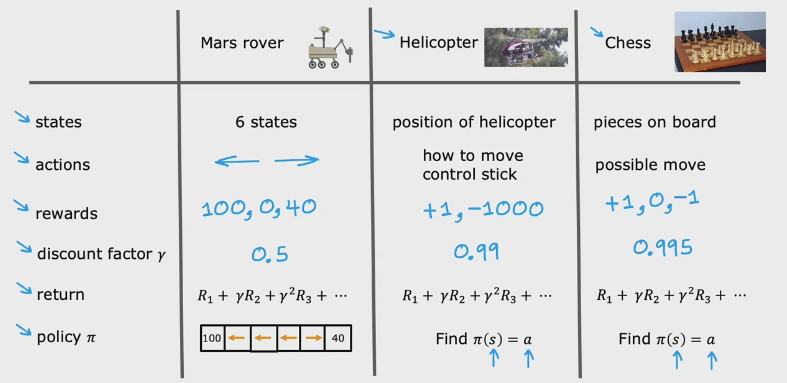
\includegraphics[width=0.82\textwidth]{source/6.png}\\
\end{center}
\end{frame}

\begin{frame}{Quá trình quyết định Markov (MDP)}{\subsecname}
\begin{itemize}
\setlength\itemsep{8pt}
\item \textbf{Quá trình ra quyết định Markov}, hay \textbf{MDP}, đề cập đến việc một kết quả nào đó trong tương lại chỉ phụ thuộc vào trạng thái hiện tại chứ không phụ thuộc vào bất kỳ điều gì có thể xảy ra trước khi đạt đến trạng thái hiện tại.\\
\vspace{8pt}
\begin{center}
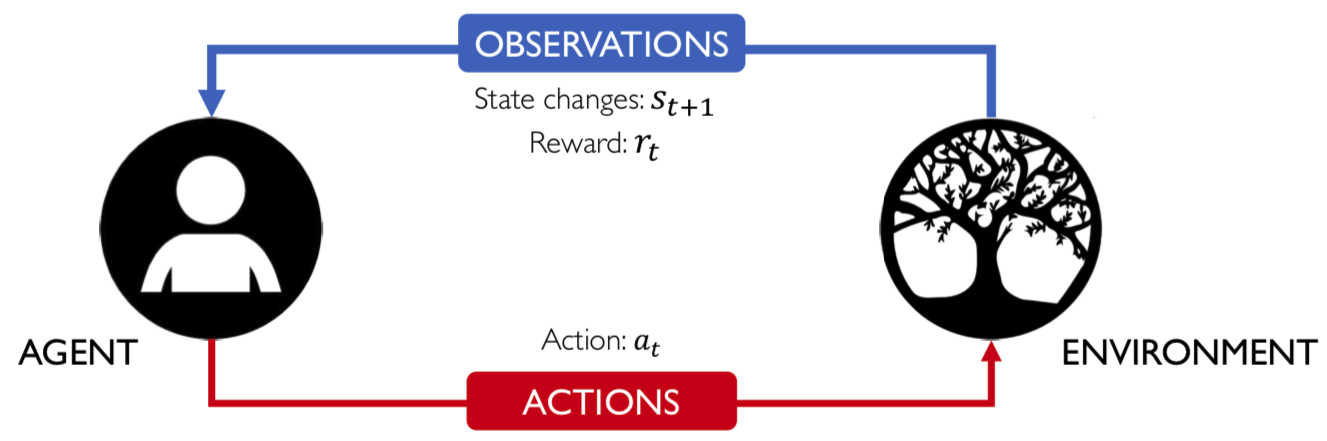
\includegraphics[width=0.5\textwidth]{source/7.png}\\
\end{center}
\item Trong RL, giả sử có một agent và ta muốn chọn các action $ a $ tác động gì đó đến environment, cách mà ta chọn action $ a $ là dựa vào policy $ \pi $ và state $ s $ của environment, và sau đó xem xét reward $ R(s) $ nhận được. Khi đó, sơ đồ thể hiện MDP được biểu diễn như hình trên.
\end{itemize}
\end{frame}

\begin{frame}{Hàm giá trị state-action}
\begin{itemize}
\setlength\itemsep{8pt}
\item \textbf{Hàm giá trị state-action $ \boldsymbol{Q(s,a)} $} là hàm của một state $ s $ mà agent có thể đang ở cùng với action $ a $ mà agent đó có thể chọn để thực hiện ở state đó.
\item \textbf{Hàm giá trị state-action $ \boldsymbol{Q(s,a)} $} trả về giá trị return, nếu agent bắt đầu ở state $ s $, thực hiện action $ a $ (chỉ một lần) và sau đó thực hiện một hành vi tối ưu nào đó, nghĩa là thực hiện bất kỳ action nào có thể mang lại giá trị return cao nhất.
\begin{equation*}
Q(s,a) = R(s) + \sum_{i=1}^{s_{terminal}} \gamma^i R(s_i) = R(s) + \gamma R(s_1) + \gamma^2 R(s_2) + ...
\end{equation*}
trong đó, $ R(s) $ là reward tại state $ s $ mà ta xét và $ s_{i} $ ($ i = \overline{1,terminal} $) là state sau khi thực hiện một hành vi tối ưu tính từ sau state $ s $.
\item Hàm giá trị state-action còn được gọi là hàm $ Q $.
\end{itemize}
\end{frame}

\begin{frame}{Hàm giá trị state-action}
\begin{center}
\textbf{Ví dụ:} Tính toán các giá trị $ Q(s,a) $ trong bài toán mô phỏng xe thám hiểm sao hoả ($ \gamma = 0.5 $): \\
\vspace{12pt}
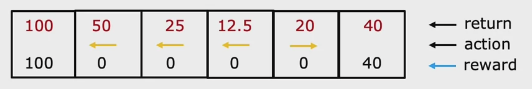
\includegraphics[width=0.5\textwidth]{source/8.png}
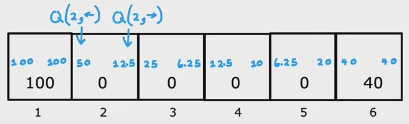
\includegraphics[width=0.5\textwidth]{source/9.png}
\begin{gather*}
Q(2,\rightarrow) = R(2) + \gamma R(3) + \gamma^2 R(2) + \gamma^3 R(1) = 0 + 0.5\times0 + 0.5^2\times0 + 0.5^3\times100 = 12.5 \\[4pt]
Q(2,\leftarrow) = R(2) + \gamma R(1) = 0 + 0.5\times100 = 50 \\[4pt]
...
\end{gather*}
\end{center}
\end{frame}

\begin{frame}{Hàm giá trị state-action}
\begin{itemize}
\setlength\itemsep{8pt}
\item Việc tính giá trị hàm $ Q $ sẽ cho ta cách chọn action $ a $ hợp lý, cụ thể giá trị return tốt nhất có thể có được từ state $ s $ là \textcolor{mainblue}{$ \max\limits_{a} Q(s,a) $}, giá trị lớn nhất của hàm $ Q(s,a) $ trên action $ a $.
\item[] $ \rightarrow $ Action $ a $ tốt nhất có thể chọn được trong state $ s $ là action $ a $ khiến giá trị hàm $ Q $ đạt \textcolor{mainblue}{$ \max\limits_{a} Q(s,a) $}
\item [] $ \rightarrow $ Hàm $ \pi(s) $ chỉ có thể chọn action $ a $ mang lại giá trị \textcolor{mainblue}{$ \max\limits_{a} Q(s,a) $}, và chắc chắn đó là một action tối ưu
\item Một số tài liệu ký hiệu hàm $ Q^* $ như là phiên bản tối ưu của hàm $ Q $, hay được gọi là hàm $ Q $ tối ưu.
\end{itemize}
\end{frame}

\begin{frame}{Phương trình Bellman}{\subsecname}
\begin{itemize}
\setlength\itemsep{8pt}
\item Trong RL, có một phương trình được gọi là \textbf{phương trình Bellman} giúp ta tính toán các giá trị $ Q(s,a) $.
\item Để mô tả phương trình Bellman. ta định nghĩa các ký hiệu:
\begin{itemize}
\setlength\itemsep{4pt}
\item[-] $ s $ và $ a $ tương ứng với state và action hiện tại
\item[-] $ R(s) $ là reward tại state hiện tại
\item[-] $ s' $ là state sau khi thực hiện action $ a $ từ state hiện tại $ s $
\item[-] $ a' $ là action mà agent có thể thực hiện ở state $ s' $
\end{itemize}
\item Phương trình Bellman: \textcolor{mainblue}{$ Q(s,a) = R(s) + \gamma\max\limits_{a'} Q(s',a') $}
\item[] \textcolor{mainblue}{\textbf{Lưu ý:}} Nếu agent đang ở state kết thúc (terminal state) thì \textcolor{mainblue}{$ Q(s,a) = R(s) $} 
\end{itemize}
\end{frame}

\begin{frame}{Môi trường ngẫu nhiên (Stochastic environment)}{\subsecname}
\begin{itemize}
\setlength\itemsep{8pt}
\item Trong một số ứng dụng, khi agent thực hiện một action, kết quả trả về không phải lúc nào cũng hoàn toàn đáng tin cậy do sự xuất hiện của một số thành phần không mong muốn từ environment
\item[] $ \longrightarrow $ Yêu cầu sự khái quát hoá mô hình RL đối với \textbf{môi trường ngẫu nhiên}
\item Trong bài toán về RL ngẫu nhiên, điều ta quan tâm là tối đa hoá giá trị trung bình của tổng số reward với yếu tố suy giảm (discount factor), thay vì tối đa hoá giá trị return do lúc này, nó chỉ là một con số ngẫu nhiên
\item[] $ \longrightarrow $ Giá trị return kì vọng (expected return) = Trung bình của các chuỗi reward khác nhau
\begin{equation*}
Expected\;return = E[R(s_1) + \gamma R(s_2) + \gamma^2 R(s_3) + ...\;]
\end{equation*}
\item[] $ \longrightarrow $ Phương trình Bellman trở thành: \textcolor{mainblue}{$ Q(s,a) = R(s) + \gamma E[\max\limits_{a'} Q(s',a')] $}
\end{itemize}
\end{frame}

\subsection{Thuật toán Reinforcement Learning}

\begin{frame}{Vùng trạng thái liên tục (Continuous state spaces)}{\subsecname}
\begin{itemize}
\setlength\itemsep{8pt}
\item Thực tế, một agent có thể có nhiều hơn một số lượng $ n $ state riêng biệt, nghĩa là nó có thể ở bất kỳ vị trí nào trong một số lượng rất lớn các giá trị liên tục.\\
\vspace{4pt}
\textcolor{mainblue2}{\textit{Chẳng hạn như một con robot có thể ở bất kỳ vị trí nào trên một đường thẳng được biểu thị bằng một số bất kỳ nằm giữa đoạn 0-6km đều hợp lệ.}}
\item Ngoài ra, còn có nhiều yếu tố tác động lên một state và tạo thành một vector (ma trận một chiều) các thuộc tính cấu thành nên một state của agent.\\
\vspace{4pt}
\textcolor{mainblue2}{\textit{Chẳng hạn như một tàu đổ bộ mặt trăng có thể có các thuộc tính bao gồm toạ độ theo phương ngang $ x $, toạ độ theo phương thẳng đứng $ y $, tốc độ di chuyển theo phương ngang $ \dot{x} $, tốc độ di chuyển theo phương thẳng đứng $ \dot{y} $, góc nghiêng $ \theta $, tốc độ nghiêng $ \dot{\theta} $, chân phải $ r $ hoặc chân trái $ l $ đã tiếp đất hay chưa, khi đó ta có state $ s $ được biểu diễn như sau:}}
\begin{equation*}
\textcolor{mainblue2}{s = [x,\;y,\;\dot{x},\;\dot{y},\;\theta,\;\dot{\theta},\;l,\;r]}
\end{equation*}
\end{itemize}
\end{frame}

\begin{frame}{Ý tưởng thuật toán}{\subsecname}
\textbf{Ý tưởng:} Huấn luyện một mạng neural để thực hiện tính toán hoặc tính gần đúng hàm giá trị state-action $ Q(s,a) $ và từ đó giúp ta chọn được các action phù hợp.\\
\begin{center}
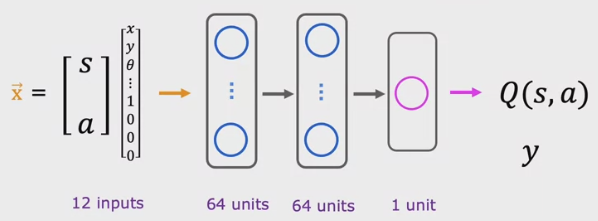
\includegraphics[width=0.8\textwidth]{source/10.png}
\end{center}
\end{frame}

\begin{frame}{Ý tưởng thuật toán}{\subsecname}
\begin{itemize}
\setlength\itemsep{8pt}
\item Đầu vào $ \vec{x} $ cho mạng neural gồm state và action hiện tại, đặt chúng lại với nhau dưới dạng vector đặc trưng một chiều.\\
\vspace{4pt}
\textcolor{mainblue2}{\textit{Đối với ví dụ về tàu đổ bộ mặt trăng, vector đặc trưng $ \vec{x} $ bao gồm 12 phần tử, trong đó 8 phần tử đầu biểu diễn cho state $ s $ và 4 phần tử sau mã hoá cho các action $ a $ có thể xảy ra.}}
\begin{equation*}
\textcolor{mainblue2}{\vec{x} = [x,\;y,\;\dot{x},\;\dot{y},\;\theta,\;\dot{\theta},\;l,\;r,\;1,\;0,\;0,\;0]}
\end{equation*}
\item Đầu ra $ y $ sau khi huấn luyện mạng neural chính là giá trị $ Q(s,a) $ được ước lượng.\\
\vspace{4pt}
\textcolor{mainblue2}{\textit{Đối với ví dụ về tàu đổ bộ mặt trăng, ta có thể sử dụng mạng neural đã được đào tạo để tính giá trị $ Q(s,a) $ ở một state $ s $ nào đó,}}
\begin{equation*}
\textcolor{mainblue2}{Q(s,\,nothing),\ Q(s,\,left),\ Q(s,\,main),\ Q(s,\,right)}
\end{equation*}
\textcolor{mainblue2}{\textit{và sau đó chọn lấy action $ a $ làm cho $ Q(s,a) $ đạt giá trị lớn nhất.}}
\end{itemize}
\end{frame}

\begin{frame}{Đào tạo hàm giá trị state-action}{\subsecname}
\begin{itemize}
\setlength\itemsep{8pt}
\item[]\begin{center}
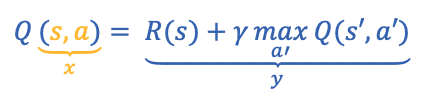
\includegraphics[width=0.4\textwidth]{source/11.png}
\end{center}
\item Để có được training dataset với các giá trị $ x $ và $ y $ để một mạng neural có thể học, nếu chua có một policy $ \pi $ tối ưu, ta sẽ thực hiện các action khác nhau (có thể tốt hoặc không) một cách ngẫu nhiên và nhiều lần, và quan sát được nhiều ví dụ ở một thời điểm mà agent đang ở một state nào đó
\item[] $ \longrightarrow $ Với mỗi state $ s $ như vậy, ta nhận được một số reward $ R(s) $
\item[] $ \longrightarrow $ Sau đó, action $ a $ nào đó vừa thực hiện sẽ đưa agent sang một state $ s' $ mới
\item Sau khi thực hiện nhiều lần, ta được một số lượng $ n $ các bộ số \textcolor{mainblue}{($ s^{(i)},\,a^{(i)},\,R(s^{(i)}),\,s'^{(i)} $)}, với $ i\;\epsilon\;[1,n] $, gọi là các \textcolor{mainblue}{\textbf{tuple}}.
\end{itemize}
\end{frame}

\begin{frame}{Đào tạo hàm giá trị state-action}{\subsecname}
\begin{itemize}
\setlength\itemsep{8pt}
\item Trong bộ số \textcolor{mainblue}{($ s^{(i)},\,a^{(i)},\,R(s^{(i)}),\,s'^{(i)} $)}, ta thấy hai phần tử đầu tiên chính là state $ s^{(i)} $ và action $ a^{(i)} $, đã quy ước là $ x^{(i)} $, và hai phần tử sau là $ R(s^{(i)}) $ và $ s'^{(i)} $, được dùng để tính ra giá trị $ y^{(i)} $ bằng cách sử dụng vế phải của phương trình Bellman.
\item[] $ \longrightarrow $ Cặp $ x^{(i)} $ và $ y^{(i)} $ được lưu lại như là một training example trong training dataset
\item Có một vấn đề là ban đầu ta không biết hàm $ Q $ là gì, do đó, những gì ta có thể bắt đầu việc đoán các giá trị của hàm này một cách hoàn toàn ngẫu nhiên.
\item[] $ \longrightarrow $ Mỗi bước thay đổi hàm $ Q $ chỉ là một giá trị phỏng đoán và hy vọng rằng nó sẽ tốt hơn theo thời gian
\item[] $ \longrightarrow $ Ta sẽ huấn luyện lại một mạng neural mới với lỗi bình phương phương trung bình (mean square error) để cố gắng dự đoán lại giá trị $ y $ với đầu vào $ x $ một cách tốt hơn
\end{itemize}
\end{frame}

\begin{frame}{Thuật toán Reinforcement Learning}
\begin{itemize}
\setlength\itemsep{8pt}
\item[Bước 1:] Khởi tạo mạng neural cùng các tất cả các tham số của mạng neural như là một dự đoán ngẫu nhiên cho hàm $ Q(s,a) $.
\item[Bước 2:] Lặp lại các bước sau cho đến khi đạt được giá trị hàm $ Q(s,a) $ tối ưu như mong muốn\\
\vspace{4pt}
\begin{itemize}
\setlength\itemsep{4pt}
\item[-] Thực hiện các action $ a $ khác nhau với các state $ s $, suy ra các tuples ($ s^{(i)},\,a^{(i)},\,R(s^{(i)}),\,s'^{(i)} $) 
\item[-] Lưu trữ khoảng 10.000 tuple $ s^{(i)},\,a^{(i)},\,R(s^{(i)}),\,s'^{(i)} $ gần nhất (relay buffer)
\item[-] Thực hiện đào tạo mạng neural:\\
\vspace{4pt}
Thiết lập training dataset gồm khoảng 10.000 training examples bằng cách định nghĩa $ x = (s,a) $ và $ y = R(s) + \gamma E[\max\limits_{a'} Q(s',a')] $, sau đó đào tạo $ Q_{new} $ sao cho $ Q_{new}(s,a) \simeq y $.
\item[-] Đặt $ Q = Q_{new} $.
\end{itemize}
\end{itemize}
$ \longrightarrow $ Thuật toán này được gọi là \textcolor{mainblue}{Mạng Q sâu (Deep Q-Network - DQN)}\footnotemark
\footnotetext[2]{V. Mnih et al., “Playing Atari with Deep Reinforcement Learning,” \textit{arXiv preprint, NIPS Deep Learning Workshop 2013}, 19 December 2013, arXiv:1312.5602.}
\end{frame}

\begin{frame}{Cải thiện kiến trúc mạng neural}{\subsecname}
Kiến trúc mạng neural đề cập tới ở trên có một vấn đề khi giả sử có $ m $ action có thể thực hiện trong một satte $ s $ thì ta phải thực hiện tính toán giá trị $ Q(s,a) $ $ m $ lần để chọn ra action mang lại giá trị $ Q(s,a) $ lớn nhất, và điều này thực sự không hiệu quả\\
\vspace{8pt}
$ \longrightarrow $ Cải tiến việc huấn luyện một mạng neural duy nhất để tính toán đồng thời ra cả $ m $ giá trị $ Q(s,a) $, và điều cần làm còn lại là chọn ra giá trị $ Q(s,a) $ lớn nhất trong số $ m $ giá trị này\\
\begin{center}
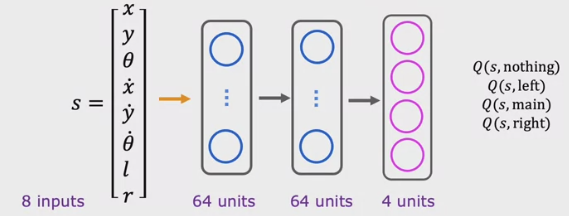
\includegraphics[width=0.6\textwidth]{source/12.png}
\end{center}
\end{frame}

\begin{frame}{$ \boldsymbol{\varepsilon} $-greedy policy}{\subsecname}
\begin{itemize}
\setlength\itemsep{8pt}
\item \textbf{$ \boldsymbol{\varepsilon} $-greedy policy} là một cách phổ biến nhất để ta có thể chọn những action tối ưu ngay trong quá trình học, bởi lẽ theo như thuật toán được đề cập ở trên, ta không thể làm điều này trừ khi đã kết thúc quá trình học.
\item \textbf{$ \boldsymbol{\varepsilon} $-greedy policy} phát biểu rằng, thay vì luôn luôn chọn ra action $ a $ mang lại giá trị $ Q(s,a) $ lớn nhất, thì ta thực hiện như sau:
\begin{itemize}
\setlength\itemsep{4pt}
\item[-] \textcolor{mainblue}{Bước khai thác (exploitation):} Trong hầu hết các trường hợp, giả sử với xác suất khoảng 0.95, ta chọn action $ a $ mang lại giá trị $ Q(s,a) $ lớn nhất (mang nghĩa tham lam (greedy))
\item[] $ \rightarrow $ Cố gắng tối đa hoá giá trị $ Q(s,a) $ bằng cách lựa chọn action tốt nhất
\item[-] \textcolor{mainblue}{Bước khám phá (exploration):} Trong một phần nhỏ trường hợp còn lại, giả sử với xác suất khoảng 0.05 ($ \varepsilon = 0.05 $), ta chọn action $ a $ một cách hoàn toàn ngẫu nhiên
\item[] $ \rightarrow $ Thử một action có thể không phải là ý tưởng tốt nhất, nhưng lại là action ta chưa có nhiều kinh nghiệm trải qua trước đây
\end{itemize}
\item Có thể bắt đầu với giá trị $ \varepsilon $ lớn, thậm chí bằng 1.0, rồi giảm dần để cải thiện hàm $ Q(s,a) $.
\end{itemize}
\end{frame}

\begin{frame}{Cập nhật theo từng mini-batch}{\subsecname}
\begin{itemize}
\setlength\itemsep{8pt}
\item \textbf{Cập nhật theo từng mini-batch} là một thuật toán giúp tăng tốc quá trình đào tạo mạng neural không chỉ trong thuật toán reinforcement learning mà còn trong các mô hình supervised learning khác.
\item Khi ta có training dataset có kích thước $ m $ rất lớn, giả sử $ m $ vào khoảng 100 triệu, thì đối với một thuật toán học máy, ví dụ như mô hình supervised learning sử dụng gradient descent, sẽ phải tính toán trung bình hơn 100 triệu training examples, sau đó ta còn phải thực hiện một bước gradient descent nhỏ rồi quay lại và quét lại toàn bộ 100 triệu training examples để tính toán trong bước tiếp theo...
\item[] $ \longrightarrow $ Điều này lặp đi lặp lại đến khi hội tụ khiến tốc độ đào tạo mạng neural chậm đi
\end{itemize}
\end{frame}

\begin{frame}{Cập nhật theo từng mini-batch}{\subsecname}
\begin{itemize}
\setlength\itemsep{8pt}
\item Ý tưởng của việc cập nhật theo từng mini-batch là không sử dụng tất cả các training examples trên mỗi lần lặp qua vòng lặp, thay vào đó, ta chọn một số lượng $ m' $ training examples nhỏ hơn $ \rightarrow $ Mỗi bước lặp lại sẽ mất ít thời gian hơn.
\item Trong mỗi lần trong mini-batch, ta sẽ ưu tiên chọn các training examples khác nhau, có thể là chọn lần lượt từ trên xuống dưới, hoặc chọn khác nhau một cách ngẫu nhiên.
\item Cụ thể trong thuật toán RL đã đề cập đến ở trên, ta thực hiện lưu trữ khoảng 10.000 tuple gần nhất (relay buffer), nhưng thay vi sử dụng toàn bộ chúng để thiết lập training dataset thì ta chỉ lấy một phần nhỏ, khoảng 1.000 tuple trong số đó, để thực hiện việc này
\item[] $ \longrightarrow $ Cách làm này sẽ làm cho mỗi lần lặp lại quá trình đào tạo mô hình sẽ ít hội tụ hơn một chút nhưng nhanh hơn nhiều, và tất nhiên vẫn hội tụ về một giá trị $ Q(s,a) $ tối ưu.
\end{itemize}
\end{frame}

\begin{frame}{\hypertarget{softupdate}{Cập nhật mềm}}{\subsecname}
\begin{itemize}
\setlength\itemsep{8pt}
\item Trong thuật toán RL đã đề cập đến ở trên, sau khi đào tạo thành công $ Q_{new} $, ta tiến hành cập nhật $ Q = Q_{new} $, tuy nhiên điều này có thể tạo ra một sự thay đổi đột ngột đối với $ Q $, thậm chí khi mạng neural đào tạo $ Q_{new} $ có thể không tốt bằng $ Q $ thì điều này sẽ khiến hệ thống trở nên tồi tệ hơn.
\item[] $ \longrightarrow $ \textbf{Cập nhật mềm (Soft updates)} là một thuật toán giúp thuật toán reinforcement learning có thể thực hiện quá trình đào tạo tốt hơn để hội tụ về một giải pháp tốt.
\item Cụ thể, mạng neural $ Q $ sẽ có một số tham số $ W $ và $ B $ môt tả các lớp trong mạng neural, khi huấn luyện mạng neural $ Q_{new} $ tương ứng có $ W_{new} $ và $ B_{new} $. Với cách thực hiện cập nhật mềm, khi cập nhật $ Q = Q_{new} $, thay vì đặt trực tiếp các tham số $ W = W_{new} $ và $ B = B_{new} $, ta sẽ đặt \textcolor{mainblue}{$ W = \alpha W_{new} + (1 - \alpha) W $} và tương ứng đối với $ B $, trong đó $ \alpha $ là một siêu tham số kiểm soát mức độ di chuyển $ W, B $ đến $ W_{new}, B_{new} $
\item[] $ \longrightarrow $ $ \alpha $ được đặt rất nhỏ, khoảng 0.01, để thực hiện thay đổi dần dần đối với các tham số của mạng neural và làm thuật toán RL hội tụ đáng tin cậy hơn.
\end{itemize}
\end{frame}

\section{Tìm hiểu về Gymnasium API}

\subsection{Cách sử dụng cơ bản}

\begin{frame}{Giới thiệu về Gymnasium API}
\begin{itemize}
\setlength\itemsep{8pt}
\item[] \begin{center}

\includegraphics[width=0.4\textwidth]{source/gymnasium-text.png}
\end{center}
\item \textcolor{mainblue}{\textbf{Gymnasium}}, hay được biết đến trước đây là \textcolor{mainblue}{\textbf{Gym}}, là một thư viện Python mã nguồn mở để phát triển và so sánh các thuật toán reinforcement learning bằng cách cung cấp API tiêu chuẩn để thực hiện giao tiếp giữa các thuật toán với hệ thống dữ liệu về môi trường đa dạng.
\item \textcolor{mainblue}{\textbf{Gymnasium}} là một nhánh được duy trì của thư viện \textcolor{mainblue}{\textbf{Gym}} của OpenAI\footnotemark, có giao diện đơn giản, phù hợp với ngôn ngữ Python, tương thích với nhiều framework học máy và có khả năng biểu thị các vấn đề liên quan đến reinforcement learning nói chung.
\end{itemize}
\footnotetext[3]{G. Brockman et al., “OpenAI Gym,” \textit{arXiv preprint}, 5 June 2016, arXiv:1606.01540.}
\end{frame}

\begin{frame}{Giới thiệu về Gymnasium API}
\begin{itemize}
\setlength\itemsep{8pt}
\item \textcolor{mainblue}{\textbf{Gymnasium}} là một dự án cung cấp API cho tất cả các môi trường reinforcement learning có agent đơn lẻ và bao gồm việc triển khai các môi trường chung: xe đẩy, con lắc, xe leo núi, mujoco, atari...
\item API của Gymnasium gồm 4 chức năng chính: \keyword{\textcolor{mainblue}{\lstinline{make}}} (tạo), \keyword{\textcolor{mainblue}{\lstinline{reset}}} (đặt lại), \keyword{\textcolor{mainblue}{\lstinline{step}}} (thực hiện từng bước) và \keyword{\textcolor{mainblue}{\lstinline{render}}} (kết xuất).
\item Cốt lõi của Gymnasium là \keyword{\textcolor{mainblue}{\lstinline{env}}}, một class Python cấp cao đại diện cho MDP từ lý thuyết reinforcement learning. Trong Gymnasium, các environment (MDPs) được triển khai dưới dạng các class \keyword{\textcolor{mainblue}{\lstinline{env}}}, cùng với \keyword{\textcolor{mainblue}{\lstinline{wrappers}}}, cung cấp các tiện ích phù hợp và có thể thay đổi kết quả được chuyển đến người dùng.
\end{itemize}
\end{frame}

\begin{frame}[fragile]{Cài đặt thư viện và API}{\subsecname}
\begin{itemize}
\setlength\itemsep{8pt}
\item Để cài đặt thư viện Gymnasium cơ bản, dùng lệnh \keyword[black]{\textcolor{gray}{\lstinline{pip install gym}}}.
\item API của Gymnasium mô hình hoá môi trường dưới dạng các class \keyword{\textcolor{mainblue}{\lstinline{env}}} đơn giản, việc tạo các phiên bản môi trường và tương tác với chúng được minh hoạ trong ví dụ dưới đây với môi trường \textbf{"CartPole-v1"}, chi tiết về cách sử dụng cơ bản được đề cập đến ở phần sau.\\
\scriptsize
\begin{lstlisting}[language=Python]
import gymnasium as gym
env = gym.make("CartPole-v1")
observation, info = env.reset(seed=42)

for _ in range(1000):
    action = env.action_space.sample()
    observation, reward, terminated, truncated, info = env.step(action)

    if terminated or truncated:
        observation, info = env.reset()
env.close()
\end{lstlisting}
\end{itemize}
\end{frame}

\begin{frame}[fragile]{Khởi tạo và tương tác với môi trường}{\subsecname}
\begin{itemize}
\setlength\itemsep{8pt}
\item Việc khởi tạo môi trường rất dễ dàng trong Gymnasium và có thể được thực hiện thông qua hàm \keyword{\textcolor{mainblue}{\lstinline{make}}}:\\
\scriptsize
\begin{lstlisting}[language=Python]
import gymnasium as gym
env = gym.make("CartPole-v1")
\end{lstlisting}
\normalsize
\item Việc này sẽ trả về \keyword{\textcolor{mainblue}{\lstinline{env}}} để người dùng tương tác. Để xem tất cả các môi trường có thể tạo, sử dụng \keyword{\textcolor{mainblue}{\lstinline{gymnasium.envs.registry.keys().make}}} bao gồm một số tham số bổ sung để thêm \keyword{\textcolor{mainblue}{\lstinline{wrappers}}}, chỉ định từ khóa cho môi trường...
\item \hyperlink{loop}{"Vòng lặp agent-environment"} cổ điển được trình bày trong lý thuyết reinforcement learning được Gymnasium triển khai một cách đơn giản hoá.
\end{itemize}
\end{frame}

\begin{frame}[fragile]{Khởi tạo và tương tác với môi trường}{\subsecname}
\begin{itemize}
\setlength\itemsep{8pt}
\item Giả sử vòng lặp được thực hiện bằng cách sử dụng đoạn code như sau:\\
\scriptsize
\begin{lstlisting}[language=Python]
import gymnasium as gym
env = gym.make("LunarLander-v2", render_mode="human")
observation, info = env.reset()

for _ in range(1000):
    # agent policy that uses the observation and info
    action = env.action_space.sample()
    observation, reward, terminated, truncated, info = env.step(action)

    if terminated or truncated:
        observation, info = env.reset()

env.close()
\end{lstlisting}
\normalsize
\item Kết quả đầu ra là một trình mô phỏng môi trường đơn giản.
\end{itemize}
\end{frame}

\begin{frame}[fragile]{Khởi tạo và tương tác với môi trường}{\subsecname}
\begin{center}
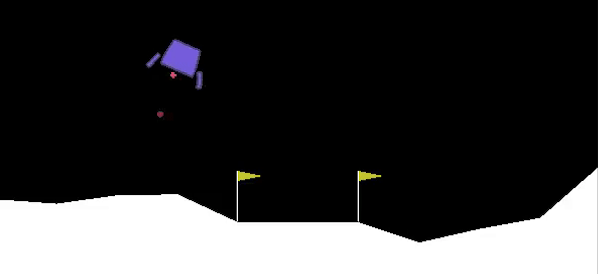
\includegraphics[width=0.88\textwidth, frame]{source/13.png}
\end{center}
\end{frame}

\begin{frame}[fragile]{Khởi tạo và tương tác với môi trường}{\subsecname}
\footnotesize
\begin{itemize}
\setlength\itemsep{8pt}
\item Đầu tiên, tạo một môi trường sử dụng \keyword{\textcolor{mainblue}{\lstinline{make}}} với từ khoá bổ sung \keyword{\textcolor{mainblue}{\lstinline{"render_mode"}}} chỉ định cách hiển thị môi trường. 
\item Sau khi khởi tạo môi trường, ta \keyword{\textcolor{mainblue}{\lstinline{reset}}} môi trường để có được observation đầu tiên. Để khởi tạo môi trường với một số tính chất nhất định hoặc tuỳ chọn ngẫu nhiên cụ thể, ta có thể sử dụng các tham số \keyword{\textcolor{mainblue}{\lstinline{seed}}} hoặc \keyword{\textcolor{mainblue}{\lstinline{options}}} với \keyword{\textcolor{mainblue}{\lstinline{reset}}}.
\item Tiếp theo, agent sẽ thực hiện một action trong môi trường, \keyword{\textcolor{mainblue}{\lstinline{step}}}, kết quả thu được là agent sẽ nhận được observation mới từ môi trường được cập nhật cùng với rewward tương ứng với action vừa thực hiện. Một lần trao đổi action-observation như vậy được gọi là một \textit{dấu thời gian (timestep)}.
\item Tuy nhiên, sau một số timestep, môi trường có thể kết thúc, lúc này được gọi là state kết thúc (terminal state). Trong Gymnasium, nếu môi trường kết thúc, nó sẽ được trả về trong \keyword{\textcolor{mainblue}{\lstinline{step}}}. Tương tự, ta cũng có thể cài đặt để môi trường kết thúc sau một số timestep cố định, khi này nó sẽ phát ra tín hiệu bị cắt ngắn (truncated signal). Nếu môi trường có \keyword{\textcolor{mainblue}{\lstinline{terminated}}} hoặc \keyword{\textcolor{mainblue}{\lstinline{truncated}}} là \keyword{\textcolor{mainblue}{\lstinline{true}}} thì nên gọi \keyword{\textcolor{mainblue}{\lstinline{reset}}} để khởi động lại môi trường.
\end{itemize}
\end{frame}

\begin{frame}{Action và observation}{\subsecname}
\begin{itemize}
\setlength\itemsep{8pt}
\item Mọi môi trường đều chỉ định định dạng của các action và observation hợp lệ với các thuộc tính \keyword{\textcolor{mainblue}{\lstinline{env.action_space}}} và \keyword{\textcolor{mainblue}{\lstinline{env.observation_space}}}. Điều này hữu ích cho cả việc biết đầu vào và đầu ra dự kiến của môi trường vì tất cả các action và observation hợp lệ phải được chứa trong không gian tương ứng.
\item Trong ví dụ trên, ta đã lấy mẫu các action ngẫu nhiên thông qua \keyword{\textcolor{mainblue}{\lstinline{env.action_space.sample()}}} ánh xạ các observation tới các action mà người dùng muốn thực hiện. 
\item Mọi môi trường đều phải có các thuộc tính \keyword{\textcolor{mainblue}{\lstinline{action_space}}} và \keyword{\textcolor{mainblue}{\lstinline{observation_space}}}, hai thuộc tính này là phiên bản của các class kế thừa từ \keyword{\textcolor{mainblue}{\lstinline{Space}}}.
\end{itemize}
\end{frame}

\begin{frame}{Action và observation}{\subsecname}
Gymnasium có hỗ trợ cho phần lớn các không gian mà người dùng có thể sử dụng:
\footnotesize
\begin{itemize}
\setlength\itemsep{4pt}
\item[-] \keyword{\textcolor{mainblue}{\lstinline{Box}}}: mô tả một không gian liên tục n chiều, giới hạn nơi ta có thể xác định giới hạn trên và giới hạn dưới mô tả các giá trị hợp lệ mà observation của ta có thể nhận được.
\item[-] \keyword{\textcolor{mainblue}{\lstinline{Discrete}}}: mô tả một không gian rời rạc trong đó \{0, 1, …, n-1\} là các giá trị có thể mà observation hoặc action của ta có thể thực hiện. Các giá trị có thể được chuyển sang \{a, a+1, …, a+n-1\} bằng cách sử dụng đối số tùy chọn.
\item[-] \keyword{\textcolor{mainblue}{\lstinline{Dict}}}: đại diện cho một từ điển của không gian đơn giản.
\item[-] \keyword{\textcolor{mainblue}{\lstinline{Tuple}}}: đại diện cho một tuple không gian đơn giản.
\item[-] \keyword{\textcolor{mainblue}{\lstinline{MultiBinary}}}: tạo ra không gian nhị phân hình chữ n (n có thể là một số hoặc một danh sách các số).
\item[-] \keyword{\textcolor{mainblue}{\lstinline{MultiDiscrete}}}: bao gồm một chuỗi các không gian chứa các action \keyword{\textcolor{mainblue}{\lstinline{Discrete}}} với số lượng action khác nhau trong mỗi phần tử.
\item[-] Ngoài ra còn có một số không gian thích hợp hơn như \keyword{\textcolor{mainblue}{\lstinline{Graph}}}, \keyword{\textcolor{mainblue}{\lstinline{Sequence}}} và \keyword{\textcolor{mainblue}{\lstinline{Text}}}.
\end{itemize}
\end{frame}

\begin{frame}[fragile]{Điều chỉnh môi trường}{\subsecname}
\begin{itemize}
\setlength\itemsep{8pt}
\item Đóng gói là một cách thuận tiện để sửa đổi môi trường hiện có mà không cần phải thay đổi code trực tiếp. Việc đóng gói giúp tránh được nhiều dạng code soạn sẵn và làm cho môi trường trở nên "module" hơn, và việc đóng gói có thể được xâu chuỗi để kết hợp các hiệu ứng giữa các "gói". Hầu hết các môi trường được tạo thông qua \keyword{\textcolor{mainblue}{\lstinline{gymnasium.make}}} sẽ được đóng gói một cách mặc định sử dụng \keyword{\textcolor{mainblue}{\lstinline{TimeLimit}}}, \keyword{\textcolor{mainblue}{\lstinline{OrderEnforcing}}} và \keyword{\textcolor{mainblue}{\lstinline{PassiveEnvChecker}}}.
\item Để đóng gói một môi trường, trước tiên ta phải khởi tạo môi trường cơ sở, sau đó chuyển môi trường này cùng với các tham số cho hàm tạo đóng gói:\\
\scriptsize
\begin{lstlisting}[language=Python]
import gymnasium as gym
from gymnasium.wrappers import FlattenObservation
env = gym.make("CarRacing-v2")
env.observation_space.shape  # >> (96, 96, 3)
wrapped_env = FlattenObservation(env)
wrapped_env.observation_space.shape  # >> (27648,)
\end{lstlisting}
\end{itemize}
\end{frame}

\begin{frame}[fragile]{Điều chỉnh môi trường}{\subsecname}
\begin{itemize}
\setlength\itemsep{8pt}
\item Gymnasium cung cấp nhiều phương thức đóng gói cho người dùng có thể sử dụng:\\
\vspace{4pt}
\footnotesize
\begin{itemize}
\setlength\itemsep{4pt}
\item[-] \keyword{\textcolor{mainblue}{\lstinline{TimeLimit}}}: phát ra tín hiệu bị cắt ngắn (truncated signal) nếu vượt quá số timestep tối đa.
\item[-] \keyword{\textcolor{mainblue}{\lstinline{ClipAction}}}: chia nhỏ action sao cho nó nằm trong không gian action (thuộc loại \keyword{\textcolor{mainblue}{\lstinline{Box}}}).
\item[-] \keyword{\textcolor{mainblue}{\lstinline{RescaleAction}}}: thay đổi tỷ lệ các action nằm trong một khoảng thời gian xác định.
\item[-] \keyword{\textcolor{mainblue}{\lstinline{TimeAwareObservation}}}: thêm thông tin về chỉ số của timestep vào observation, trong một số trường hợp hữu ích để đảm bảo rằng quá trình chuyển đổi là Markov.
\end{itemize}
\normalsize
\item Thuộc tính \keyword{\textcolor{mainblue}{\lstinline{.unwrapped}}} để đưa một môi trường về trạng thái chưa đóng gói, để ta có thể gọi một hàm nào đó thủ công hoặc thay đổi một số khía cạnh của môi trường.\\
\scriptsize
\begin{lstlisting}[language=Python]
wrapped_env
# >> <FlattenObservation<TimeLimit<OrderEnforcing<PassiveEnvChecker<CarRacing<CarRacing-v2>>>>>>
wrapped_env.unwrapped
# >> <gymnasium.envs.box2d.car_racing.CarRacing object at 0x7f04efcb8850>
\end{lstlisting}
\end{itemize}
\end{frame}

\subsection{Một số khái niệm cơ bản về Gymnasium}

\begin{frame}{Giới hạn thời gian xử lý}{\subsecname}
Khi sử dụng môi trường Gymnasium để triển khai reinforcement learning, một vấn đề thường gặp là việc xử lý thời gian không chính xác. Tín hiệu \keyword{\textcolor{mainblue}{\lstinline{done}}} nhận được từ \keyword{\textcolor{mainblue}{\lstinline{env.step}}} cho biết một quá trình đã kết thúc hay chưa, nhưng lại không phân biệt được nó kết thúc do \keyword{\textcolor{mainblue}{\lstinline{termination}}} hay \keyword{\textcolor{mainblue}{\lstinline{truncation}}}.\\
\vspace{4pt}
\footnotesize
\begin{itemize}
\setlength\itemsep{4pt}
\item[-] \keyword{\textcolor{mainblue}{\lstinline{termination}}} biểu diễn cho quá trình kết thúc \textcolor{mainblue}{\textbf{sau khi đạt đến state kết thúc được xác định như một phần định nghĩa sẵn từ môi trường}}.\\
\vspace{2pt}
\keyword{\textcolor{mainblue}{\lstinline{termination}}} cũng bao gồm quá trình kết thúc trong một \textcolor{mainblue}{\textbf{môi trường hữu hạn}} do giới hạn thời gian (trường hợp này cần có biểu diễn thời gian còn lại trong obsservation của agent để bảo toàn thuộc tính Markov).
\item[-] \keyword{\textcolor{mainblue}{\lstinline{truncation}}} biểu diễn cho quá trình kết thúc \textcolor{mainblue}{\textbf{sau một điều kiện được xác định bên ngoài phạm vi của MDP}}, nó có thể là giới hạn thời gian, hoặc khi agent đi ra khỏi giới hạn nào đó...\\
\vspace{2pt}
\keyword{\textcolor{mainblue}{\lstinline{truncation}}} thường được sử dụng trong các \textcolor{mainblue}{\textbf{môi trường vô hạn}}, khi ta không thể đợi cho đến khi môi trường kết thúc nên phải đặt ta một giới hạn thời gian để tạm dừng quá trình (trường hợp này có state cuối cùng không phải state kết thúc vì nó có xác suất chuyển tiếp khác 0 để chuyển sang state khác theo MDP).
\end{itemize}
\end{frame}

\begin{frame}{Giới hạn thời gian xử lý}{\subsecname}
\begin{itemize}
\setlength\itemsep{8pt}
\item Bootstrapping (khởi động), việc sử dụng một hoặc nhiều giá trị ước tính của một biến để cập nhật các ước tính của chính biến đó, là một khía cạnh quan trọng của reinforcement learning. Hàm giá trị sẽ cho biết agent sẽ nhận được bao nhiêu reward từ một state cụ thể nếu tuân theo một policy nhất định.\\
\vspace{4pt}
Điều này có nghĩa là khi một quá trình dừng ở bất kỳ điểm nào, bằng cách xem xét giá trị của state cuối cùng, agent có thể ước tính được reward có thể nhận được nếu quá trình đó tiếp tục.
\item Một ví dụ phổ biến về bootstrapping trong RL là cập nhật giá trị ước tính của hàm $ Q $, có phương trình $ Q(s,a) = R(s) + \gamma\max\limits_{a'} Q(s',a') $.\\
\vspace{4pt}
Trong RL, ước tính \keyword{\textcolor{mainblue}{\lstinline{Q}}} mới là trung bình có trọng số của ước tính \keyword{\textcolor{mainblue}{\lstinline{Q}}} trước đó và \keyword{\textcolor{mainblue}{\lstinline{Q_target}}} (\hyperlink{softupdate}{thuật toán cập nhật mềm}), khi đó, sai số giữa \keyword{\textcolor{mainblue}{\lstinline{Q_target}}} và ước tính \keyword{\textcolor{mainblue}{\lstinline{Q}}} trước đó được giảm thiểu.
\end{itemize}
\end{frame}

\begin{frame}[fragile]{Giới hạn thời gian xử lý}{\subsecname}
\begin{itemize}
\setlength\itemsep{8pt}
\item Tuy nhiên, ở state kết thúc, bootstrapping không thực hiện và trả về $ Q(s,a) = R(s) $.\\
\vspace{4pt}
Đây là nơi sự khác biệt giữa \keyword{\textcolor{mainblue}{\lstinline{termination}}} và \keyword{\textcolor{mainblue}{\lstinline{truncation}}} đặc biệt quan trọng. Cụ thể, khi một quá trình kết thúc do \keyword{\textcolor{mainblue}{\lstinline{termination}}}, ta không thực hiện bootstrap, còn khi quá trình kết thúc do \keyword{\textcolor{mainblue}{\lstinline{truncation}}}, ta thực hiện bootstrap.
\item Khi sử dụng môi trường Gymnasium, tín hiệu \keyword{\textcolor{mainblue}{\lstinline{done}}} thường được sử dụng để xác định xem có nên thực hiện bootstrap hay không, tuy nhiên nó lại không chính xác vì không phân biệt được \keyword{\textcolor{mainblue}{\lstinline{termination}}} và \keyword{\textcolor{mainblue}{\lstinline{truncation}}}.
\item[] $ \longrightarrow $ Thay vì sử dụng \keyword{\textcolor{mainblue}{\lstinline{done}}}, API \keyword{\textcolor{mainblue} {\lstinline{env.step}}} của Gymnasium sẽ trả về cả thông tin của \keyword{\textcolor{mainblue}{\lstinline{termination}}} và \keyword{\textcolor{mainblue}{\lstinline{truncation}}} một cách rõ ràng. Như vậy, cách chính xác nhất để xử lý \keyword{\textcolor{mainblue}{\lstinline{termination}}} và \keyword{\textcolor{mainblue}{\lstinline{truncation}}} bây giờ là,\\
\scriptsize
\begin{lstlisting}[language=Python]
# INCORRECT: vf_target = rew + gamma * (1 - done) * vf_next_state
vf_target = rew + gamma * (1 - terminated) * vf_next_state
\end{lstlisting}
\end{itemize}
\end{frame}

\begin{frame}[fragile]{Kế thừa từ \keyword{\textcolor{mainblue}{\lstinline{gymnasium.ObservationWrapper}}}}
\framesubtitle{Triển khai các gói tùy chỉnh}
\begin{itemize}
\setlength\itemsep{4pt}
\footnotesize
\item \keyword{\textcolor{mainblue}{\lstinline{ObservationWrapper}}} hữu ích khi ta muốn áp dụng một số hàm cho các observation dược môi trường trả về. Ta triển khai \keyword{\textcolor{mainblue}{\lstinline{ObservationWrapper}}} bằng \keyword{\textcolor{mainblue}{\lstinline{gymnasium.ObservationWrapper.observation()}}}. Lưu ý rằng ta cần cập nhật không gian observation nếu phép biến đổi làm thay đổi hình dạng của observation.
\item Giả sử có một tác vụ điều hướng 2D trong đó môi trường trả về từ điển chứa các observation dưới dạng các từ khoá \keyword{\textcolor{mainblue}{\lstinline{"agent_position"}}} và \keyword{\textcolor{mainblue}{\lstinline{"target_position"}}}. Một điều phổ biến cần làm là loại bỏ một số thành phần tự do và chỉ xem xét đến \keyword{\textcolor{mainblue}{\lstinline{obs["agent_position"] - obs["target_position"]}}}.\\
\scriptsize
\begin{lstlisting}[language=Python]
import numpy as np
import gymnasium as gym
from gym import ActionWrapper, ObservationWrapper, RewardWrapper, Wrapper
from gymnasium.spaces import Box, Discrete

class RelativePosition(ObservationWrapper):
    def __init__(self, env):
        super().__init__(env)
        self.observation_space = Box(shape=(2,), low=-np.inf, high=np.inf)

    def observation(self, obs):
        return obs["target"] - obs["agent"]
\end{lstlisting}
\end{itemize}
\end{frame}

\begin{frame}[fragile]{Kế thừa từ \keyword{\textcolor{mainblue}{\lstinline{gymnasium.ActionWrapper}}}}
\framesubtitle{Triển khai các gói tùy chỉnh}
\begin{itemize}
\setlength\itemsep{4pt}
\footnotesize
\item \keyword{\textcolor{mainblue}{\lstinline{ActionWrapper}}} hữu ích khi ta muốn áp dụng một số thay đổi cho action trước khi áp dụng chúng vào môi trường. Ta triển khai \keyword{\textcolor{mainblue}{\lstinline{ActionWrapper}}} bằng \keyword{\textcolor{mainblue}{\lstinline{gymnasium.ActionWrapper.action()}}}. Lưu ý rằng ta nên chỉ định miền của phép thay đổi bằng cách cập nhật không gian action.
\item Giả sử có một môi trường có không gian action thuộc loại \keyword{\textcolor{mainblue}{\lstinline{gymnasium.spaces.Box}}} nhưng ta lại chỉ muốn sử dụng một tập con các action thì ta thực hiện như sau:
\tiny
\begin{lstlisting}[language=Python]
class DiscreteActions(ActionWrapper):
    def __init__(self, env, disc_to_cont):
        super().__init__(env)
        self.disc_to_cont = disc_to_cont
        self.action_space = Discrete(len(disc_to_cont))

    def action(self, act):
        return self.disc_to_cont[act]

if __name__ == "__main__":
    env = gym.make("LunarLanderContinuous-v2")
    wrapped_env = DiscreteActions(
        env, [np.array([1, 0]), np.array([-1, 0]), np.array([0, 1]), np.array([0, -1])]
    )
    print(wrapped_env.action_space)  # Discrete(4)
\end{lstlisting}
\end{itemize}
\end{frame}

\begin{frame}[fragile]{Kế thừa từ \keyword{\textcolor{mainblue}{\lstinline{gymnasium.RewardWrapper}}}}
\framesubtitle{Triển khai các gói tùy chỉnh}
\begin{itemize}
\setlength\itemsep{4pt}
\item \keyword{\textcolor{mainblue}{\lstinline{RewardWrapper}}} hữu ích khi ta thay đổi reward được môi trường trả về. Ta triển khai \keyword{\textcolor{mainblue}{\lstinline{RewardWrapper}}} bằng \keyword{\textcolor{mainblue}{\lstinline{gymnasium.RewardWrapper.reward()}}}. Ngoài ra, ta có thể cập nhật phạm vi rewward của "gói".
\item Giả sử đôi khi (đặc biệt là khi ta không có quyền kiểm soát reward), ta muốn chia reward vào một phạm vi nào đó để đạt được sự ổn định về số lượng thì ta thực hiện như sau:
\scriptsize
\begin{lstlisting}[language=Python]
from typing import SupportsFloat

class ClipReward(RewardWrapper):
    def __init__(self, env, min_reward, max_reward):
        super().__init__(env)
        self.min_reward = min_reward
        self.max_reward = max_reward
        self.reward_range = (min_reward, max_reward)

    def reward(self, r: SupportsFloat) -> SupportsFloat:
        return np.clip(r, self.min_reward, self.max_reward)
\end{lstlisting}
\end{itemize}
\end{frame}

\begin{frame}[fragile]{Kế thừa từ \keyword{\textcolor{mainblue}{\lstinline{gymnasium.Wrapper}}}}
\framesubtitle{Triển khai các gói tùy chỉnh}
\begin{itemize}
\setlength\itemsep{8pt}
\item Đôi khi, ta có thể cần triền khai \keyword{\textcolor{mainblue}{\lstinline{Wrapper}}} thực hiện một số thay đổi phức tạp hơn, chẳng hạn như thay đổi reward dựa trên dữ liệu hoặc thay đổi hành vi hiển thị. Các \keyword{\textcolor{mainblue}{\lstinline{Wrapper}}} như vậy có thể được triển khai bằng cách kế thừa \keyword{\textcolor{mainblue}{\lstinline{gymnasium.Wrapper}}}.
\vspace{4pt}
\begin{itemize}
\setlength\itemsep{4pt}
\item[-] Ta có thể đặt một không gian cho action hoặc observation bằng cách định nghĩa \keyword{\textcolor{mainblue}{\lstinline{self.action_space}}} hoặc \keyword{\textcolor{mainblue}{\lstinline{self.observation_space}}} trong \keyword{\textcolor{mainblue}{\lstinline{__init__}}}
\item[-] Ta có thể đặt một dữ liệu và một phạm vi rewward mới bằng cách định nghĩa \keyword{\textcolor{mainblue}{\lstinline{self.metadata}}}  \keyword{\textcolor{mainblue}{\lstinline{self.reward_range}}} trong \keyword{\textcolor{mainblue}{\lstinline{__init__}}}
\item[-] Thậm chí ta có thể ghi đè \keyword{\textcolor{mainblue}{\lstinline{gymnasium.Wrapper.step()}}}, \keyword{\textcolor{mainblue}{\lstinline{gymnasium.Wrapper.render()}}}, \keyword{\textcolor{mainblue}{\lstinline{gymnasium.Wrapper.close()}}}...
\end{itemize}
\item Sau đó, ta có thể truy cập vào môi trường đã được chuyển vào trong \keyword{\textcolor{mainblue}{\lstinline{Wrapper}}} bằng cách truy cập thuộc tính \keyword{\textcolor{mainblue}{\lstinline{env}}}.
\end{itemize}
\end{frame}

\begin{frame}[fragile]{Kế thừa từ \keyword{\textcolor{mainblue}{\lstinline{gymnasium.Wrapper}}}}
\framesubtitle{Triển khai các gói tùy chỉnh}
\footnotesize
Giả sử trong môi trường MuJoCo\footnotemark, có một quy định nào đó về reward cho agent hoàn thành nhiệm vụ và hình phạt cho agent nếu phạm lỗi lớn. Thông thường, ta có thể truyền vào các tham số trọng số cho các quy định đó trong quá trình khởi tạo môi trường, tuy nhiên Reacher\footnotemark \hspace{1pt} lại không cho phép làm điều này.\\
\vspace{4pt}
Giải pháp là xây dưng một \keyword{\textcolor{mainblue}{\lstinline{Wrapper}}} cho Reacher để cho phép ta tính trọng số các quy định đó.\\
\vspace{8pt}
\scriptsize
\begin{lstlisting}[language=Python]
class ReacherRewardWrapper(Wrapper):
    def __init__(self, env, reward_dist_weight, reward_ctrl_weight):
        super().__init__(env)
        self.reward_dist_weight = reward_dist_weight
        self.reward_ctrl_weight = reward_ctrl_weight

    def step(self, action):
        obs, _, terminated, truncated, info = self.env.step(action)
        reward = (
            self.reward_dist_weight * info["reward_dist"]
            + self.reward_ctrl_weight * info["reward_ctrl"]
        )
        return obs, reward, terminated, truncated, info
\end{lstlisting}
\footnotetext[4]{\url{https://www.gymlibrary.dev/environments/mujoco/}}
\footnotetext[5]{\url{https://www.gymlibrary.dev/environments/mujoco/reacher/}}
\end{frame}

\begin{frame}[fragile]{Tạo môi trường tùy chỉnh}{\subsecname}
\begin{itemize}
\setlength\itemsep{8pt}
\item Tham khảo trong \href{https://gymnasium.farama.org/tutorials/gymnasium_basics/environment_creation/#sphx-glr-tutorials-gymnasium-basics-environment-creation-py}{Gymnasium Basics | Make your own custom environment}
\item Thực hành trong Jupyter Notebook
\end{itemize}
\end{frame}

\section{Kết luận}

\begin{frame}{Kết luận}
\begin{itemize}
\setlength\itemsep{8pt}
\item \textbf{\textcolor{mainblue}{Reinforcement learning}} là phương pháp đào tạo các mô hình học máy để đưa ra một chuỗi các quyết định hay hành động phù hợp để đạt được kết quả tốt nhất trong một tình huống cụ thể. Nhiệm vụ của thuật toán \textbf{\textcolor{mainblue}{reinforcement learning}} là tìm ra cách thu được nhiều kết quả tốt hơn và ít kết quả xấu.
\item \textbf{\textcolor{mainblue}{Gymansium}} là một thư viện Python mã nguồn mở để phát triển và so sánh các thuật toán reinforcement learning bằng cách cung cấp API tiêu chuẩn để thực hiện giao tiếp giữa các thuật toán với hệ thống dữ liệu về môi trường đa dạng.
\item Thực hành sử dụng cơ bản với một số khái niệm và API của \textbf{\textcolor{mainblue}{Gymansium}}.
\end{itemize}
\end{frame}

\backmatter

\end{document}